\documentclass[11pt,slides,aspectratio=43]{beamer}%
\usepackage[utf8]{inputenc}
\usepackage[russian]{babel}
\usepackage{multicol}
\usepackage{ragged2e}

\usepackage{amsmath}
\usepackage{amsfonts}
\usepackage{amssymb}
\usepackage{amsthm}

\usepackage{newlfont}
\usepackage{graphics}
\usepackage[perpage]{footmisc}

\setbeamertemplate{navigation symbols}{} % отключаем клавиши навигации

\usepackage{xcolor}
\usepackage{hyperref} % гиперссылки в пдф-ке
\definecolor{linkcolor}{HTML}{000010} % цвет ссылок
\definecolor{urlcolor}{HTML}{001488} % цвет гиперссылок
\hypersetup{pdfstartview=FitH,  linkcolor=linkcolor, urlcolor=urlcolor, colorlinks=true}


\usetheme{CambridgeUS} %CambridgeUS %Dresden %Warsaw %Madrid
%\usecolortheme{dolphin}%dolphin
%\usecolortheme[RGB={0, 110, 25}]{structure} %wolverine %whale
%\beamertemplatetransparentcovereddynamicmedium
\beamertemplateshadingbackground{white!25}{white!35}
%\beamertemplategridbackground[15]

\title{$\mu$Notes}
%\author[]{Доммес В., Кривошеин С., Поляков Д. \\ Куратор: Тузова Е., JetBrains}
\author[]{Василий Доммес, Сергей Кривошеин, Денис Поляков
	\\ Куратор: Екатерина Тузова, JetBrains}

\date{18 декабря 2014 г.}

\begin{document}

	\begin{frame}
		\maketitle
	\end{frame}

    \begin{frame}{Цели работы}
		\begin{itemize}
            \item Получение нотной записи музыкального трека
            \item В записи могут присутствовать чистые инструменты (фортепиано, акустическая гитара...)
        \end{itemize}
	\end{frame}

    \begin{frame}{Предмет поиска}
        \begin{figure}[h!]
            \begin{center}
                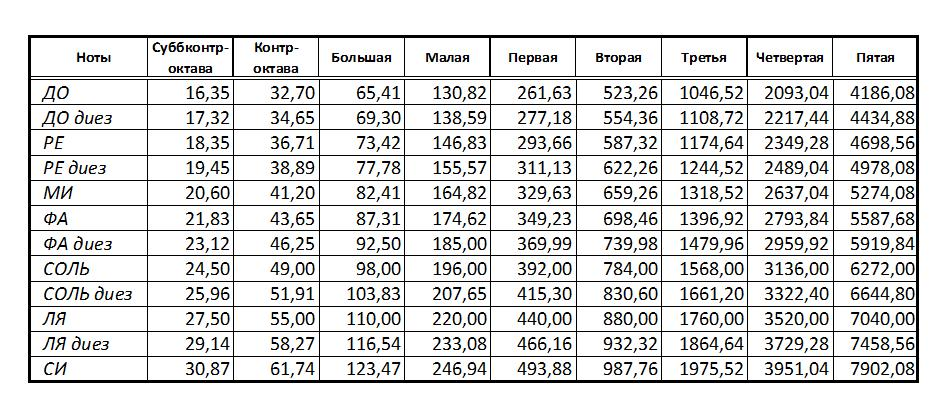
\includegraphics[width = 0.85\textwidth]{notes.jpg}
                %\caption{Ноты девяти октав}
            \end{center}
        \end{figure}
        \begin{center}
           Частоты нот [Гц]
        \end{center}
    \end{frame}

    \begin{frame}{Представление звукового сигнала.}
        \begin{figure}[h!]
            \begin{center}
                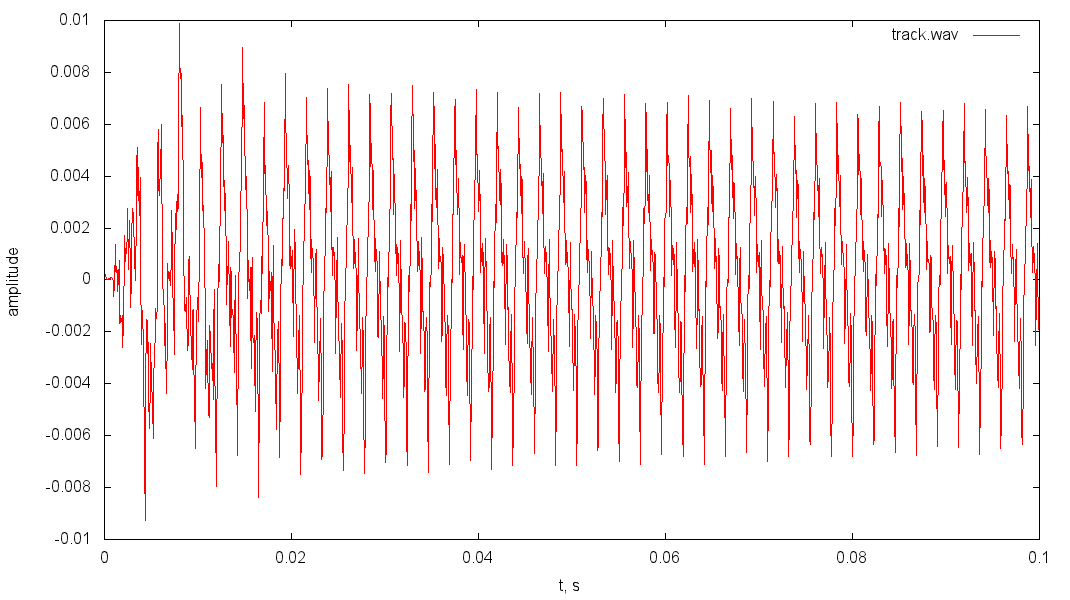
\includegraphics[width = 0.85\textwidth]{series.png}
                %\caption{Нота Ля}
            \end{center}
        \end{figure}
        \begin{center}
           Нота Ля
        \end{center}
    \end{frame}

    \begin{frame}{Алгоритм построения нотной записи}
        \begin{itemize}
            \item Построение динамического спектра исходного звукового сигнала с помощью STFT
            \item Построение вторичного спектра по первичному с помощью вейвлет-преобразования.
            \item Взаимный анализ двух получившихся спектров.
            \item Получение функции вероятности звучания ноты в каждый момент времени.
        \end{itemize}
    \end{frame}

    \begin{frame}{Первичный спектр}
        \begin{figure}[h!]
            \begin{center}
                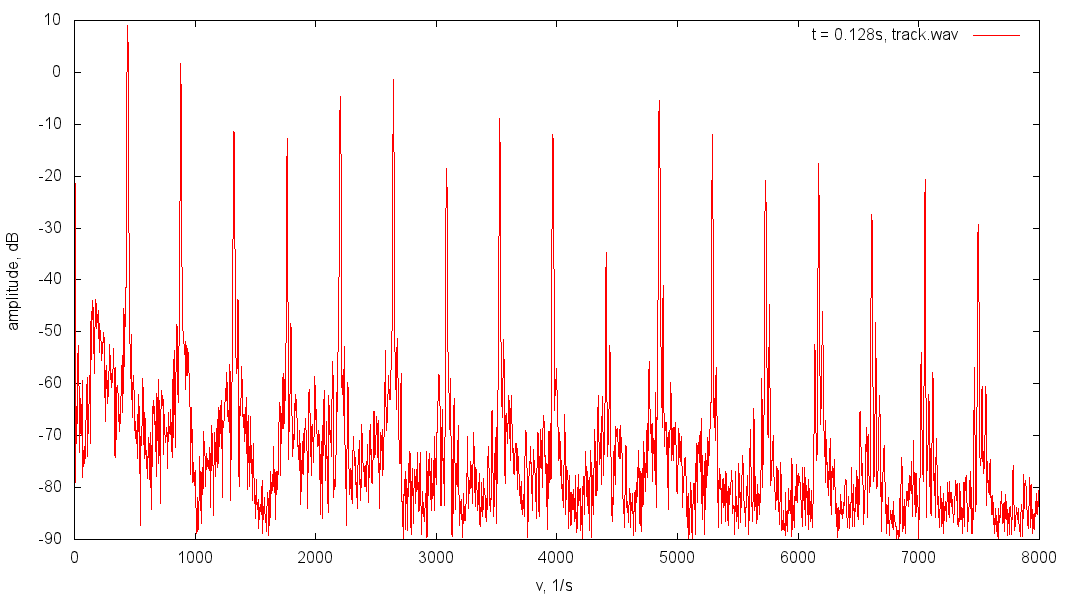
\includegraphics[width = 0.85\textwidth]{firstSpectrum.png}
                %\caption{Срез динамический спектра}
            \end{center}
        \end{figure}
        \begin{center}
           Срез динамического спектра
        \end{center}
    \end{frame}

    \begin{frame}{Свёртка первичного спектра}
        \begin{itemize}
            \item В первичном спектре реального звука есть много шумов и артефактов(обертона).
            \item Проблема усугубляется при звучании множества нот одновременно, особенно, когда они отличаются на октаву.
            \item Решение -- свёртка первичного спектра с вейвлетом. При этом выделяется основной тон и исчезают обертона.
        \end{itemize}
    \end{frame}

    \begin{frame}{Вторичный спектр}
        \begin{figure}[h!]
            \begin{center}
                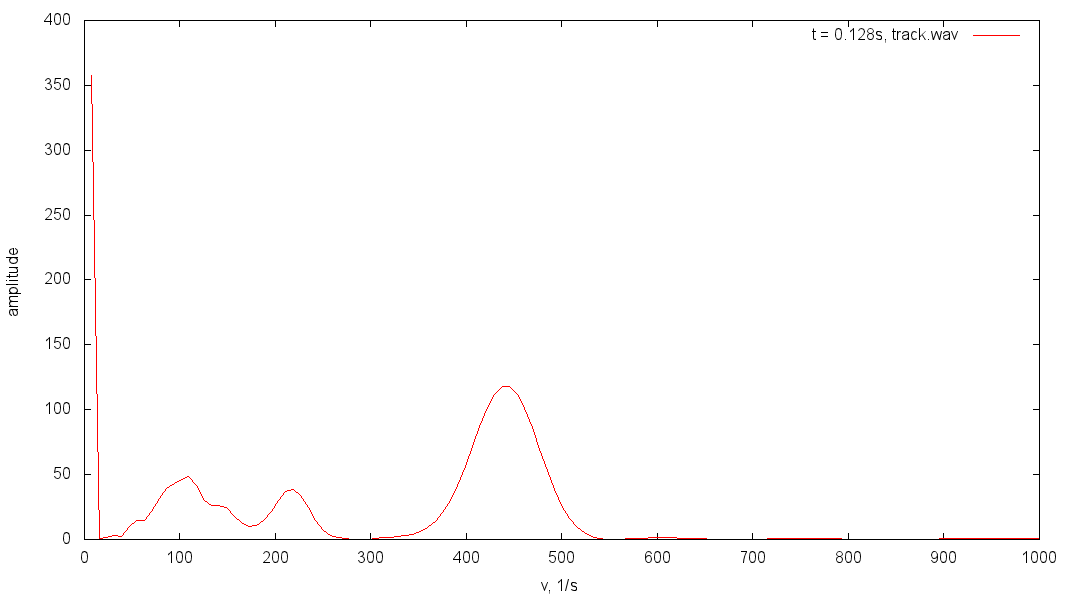
\includegraphics[width = 0.85\textwidth]{secondSpectrum.png}
                %\caption{Срез вторичного вейвлет-спектра}
            \end{center}
        \end{figure}
        \begin{center}
           Срез вторичного вейвлет-спектра
        \end{center}
    \end{frame}

    \begin{frame}{Фурье-преобразование}
        $$
        \varphi(\nu) = e^{-i 2 \pi \nu t}
        $$
        \begin{figure}[h!]
            \begin{center}
                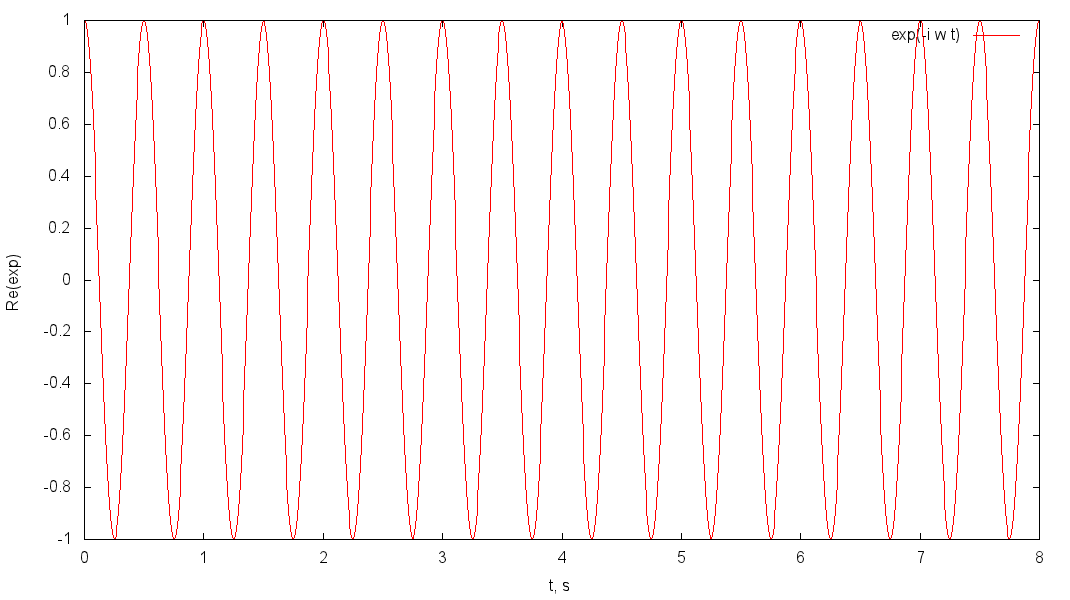
\includegraphics[width = 0.5\textwidth]{exp.png}
                %\caption{Базисная функция Фурье-преобразования (вещественная часть)}
            \end{center}
        \end{figure}
        \begin{center}
           Базисная функция Фурье-преобразования (вещественная часть)
        \end{center}
        $$
        \mbox{Преобразование Фурье ~~~}\widehat{f} = \int\limits_{-\infty}^{\infty} f(t) e^{-i 2 \pi \nu t} dt
        $$
    \end{frame}

    \begin{frame}{Периодограмма}
    %\frametitle{Люди подарившие нам нейтронные звёзды.}
    В случае, когда сигнал представляется дискретным временным рядом, вместо спектра используется периодограмма
    $$
        D(\nu) = \frac{1}{N^{2}}\left|\sum\limits_{k = 0}^{N - 1} x_{k} e^{-i 2 \pi \nu t_{k}} \right|^{2}
    $$
    В основе вычисления периодограммы стоит DFT.
    \vskip2pt
    При вычислении периодограммы на фундаментальной системе частот используется FFT
    \end{frame}

    \begin{frame}
	\frametitle{Основные особенности периодограммы}
        \begin{figure}[h!]
            \begin{center}
                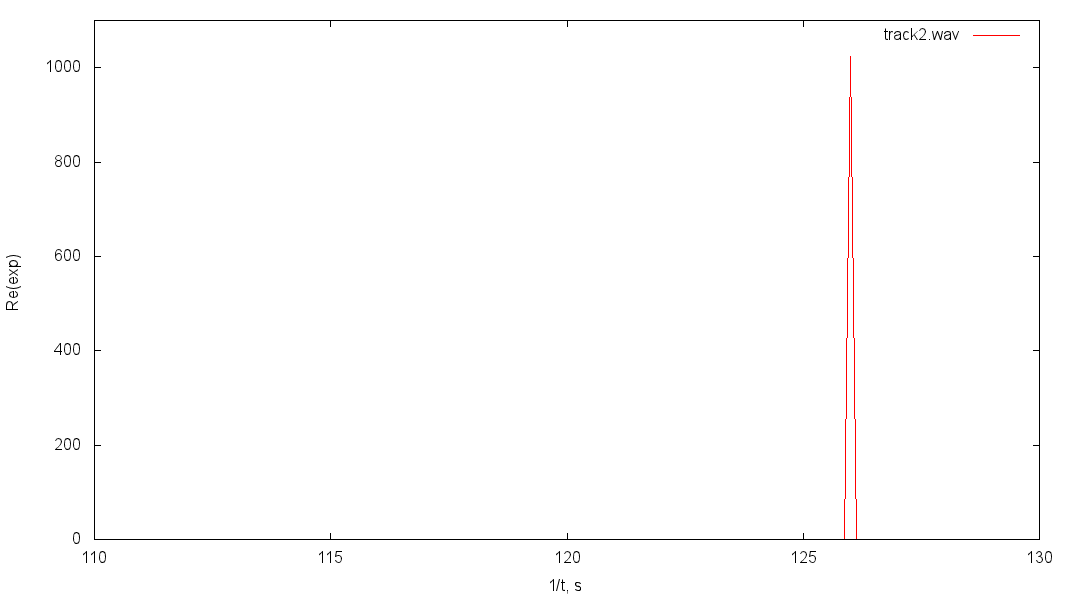
\includegraphics[width = 0.5\textwidth]{spec1.png}
                \caption{Периодограмма синусоидального сигнала}
            \end{center}
        \end{figure}
	   \begin{block}{}
            \begin{itemize}
	           \item Лучший инструмент для извлечения периодических компонент из сигнала.
	           \item Чувствителен к полиномиальной составляющей(трендам).
            \end{itemize}
		\end{block}
	\end{frame}

    \begin{frame}{STFT}
        \begin{itemize}
	           \item Для получения динамического спектра необходимо применять процедуру FFT к <<небольшим>> участкам нашего спектра.
	           \item В качестве инструмента рассмотрим свёртку с окном Блэкмана--Харриса
        \end{itemize}

        $$
            W(x) = 0.42 - 0.5 \cos(2 \pi x) + 0.08 cos(4 \pi x)
        $$

    \end{frame}

    \begin{frame}
        \begin{figure}[h!]
            \begin{center}
                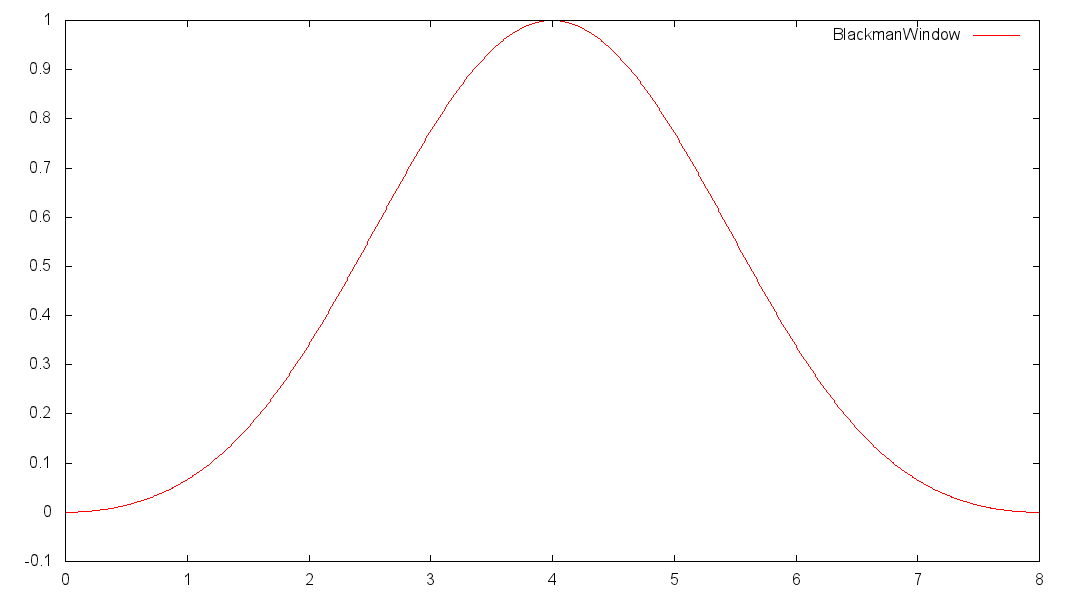
\includegraphics[width = 0.85\textwidth]{window.png}
                %\caption{Окно Блэкмана}
            \end{center}
        \end{figure}
        \begin{center}
            Окно Блэкмана
        \end{center}
    \end{frame}

    \section{Вейвлеты}

    \begin{frame}
	\frametitle{Вейвлет}
	   Интегральное вейвлет-преобразование функции $f(t)$
    $$
        W(a, b) = \frac{1}{\left|a\right|^{2}} \int\limits_{-\infty}^{\infty} f(t) \psi(\frac{t - b}{a}) dt,
    $$
    $a$ - масштаб, $b$ - сдвиг, $\psi(t)$ -- базисный вейвлет
    \vskip2pt
	\end{frame}
	
    \begin{frame}
	\frametitle{Вейвлет Морле}
    ~~~~~~Вейвлет Морле -- плоская волна модулированная гауссианой.
    $$
        \psi(t) = e^{-t^{2} / \alpha^{2}}\left[e^{i k_{0} t} - e^{-k_{0}^{2}\alpha^{2}/4}\right]
    $$
    Параметр $\alpha$ задаёт ширину гауссианы, параметр $k_{0}$ -- частоту плоской волны
	\end{frame}

    \begin{frame}
        \begin{figure}[h!]
            \begin{center}
                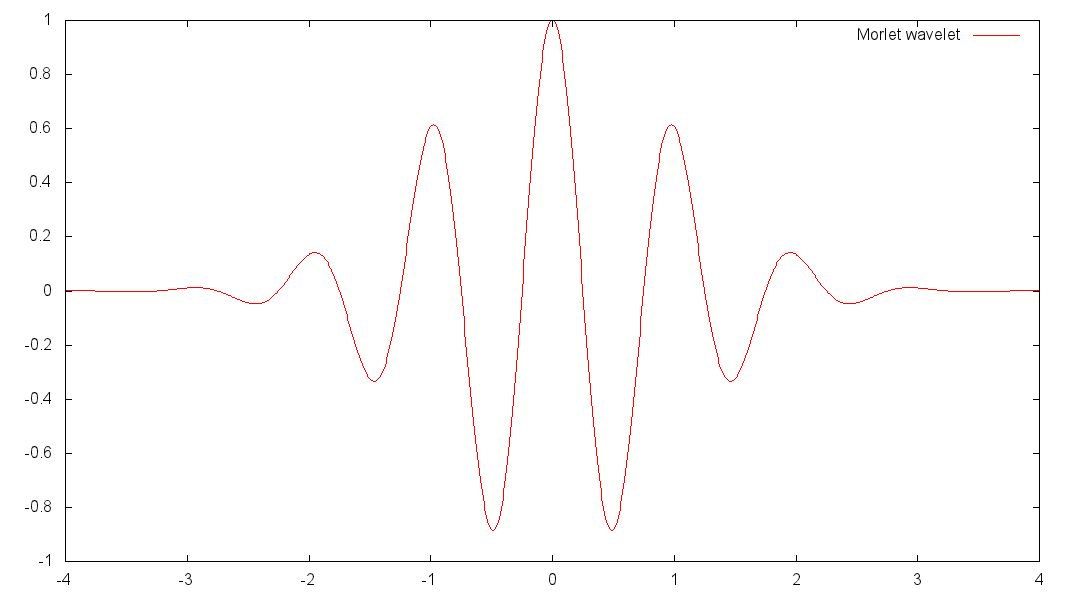
\includegraphics[width = 0.5\textwidth]{wavelet.png}
                %\caption{Базисная функция вейвлета Морле при $\alpha^{2} = 2, k_{0} = 2 \pi$}
            \end{center}
            \begin{center}
                Базисная функция вейвлета Морле при $\alpha^{2} = 2, k_{0} = 2 \pi$
            \end{center}
        \end{figure}
        \begin{figure}[h!]
            \begin{center}
                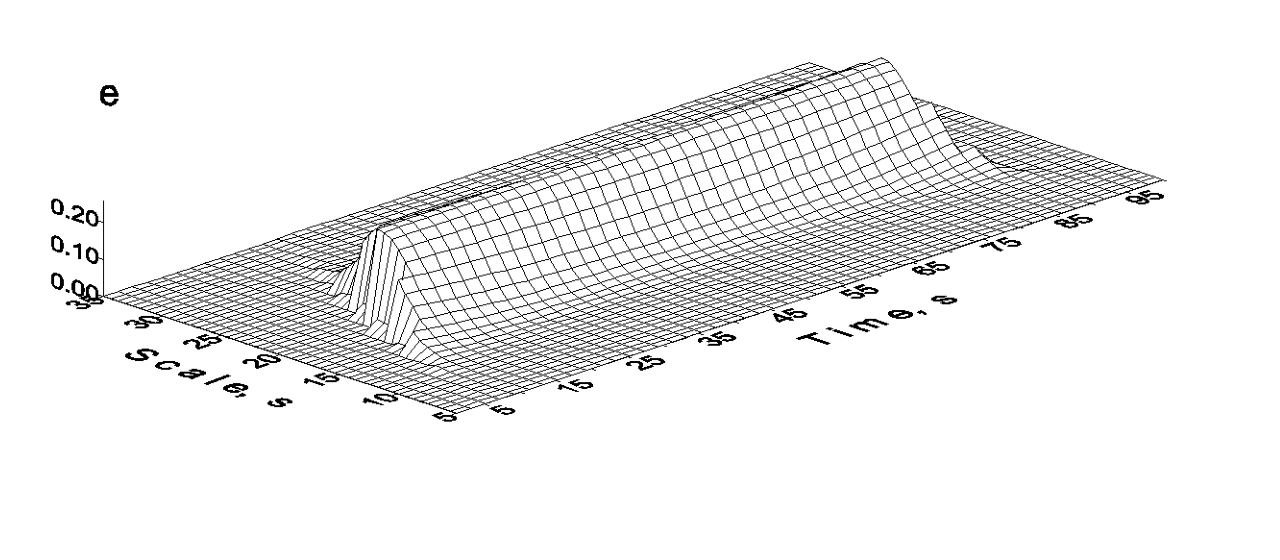
\includegraphics[width = 0.5\textwidth]{323.png}
                %\caption{Интегральное вейвлет-преобразование синусоидального сигнала}
            \end{center}
            \begin{center}
                Интегральное вейвлет-преобразование синусоидального сигнала
            \end{center}
        \end{figure}
    \end{frame}

    \begin{frame}
	\frametitle{Основные особенности вейвлета}
	   \begin{block}{}
            \begin{itemize}
	           \item Хорошая временная и частотная локализация.
	           \item Чувствителен к полиномиальной составляющей(трендам).
               \item При неортогональном наборе базисных вейвлетов нет быстрого преобразования.
            \end{itemize}
		\end{block}
	\end{frame}

    \begin{frame}
    \frametitle{Результаты}
               ~~~~~~~~~~ Аккорды, взятые на акустической гитаре.
	   \begin{figure}[h!]
            \begin{center}
                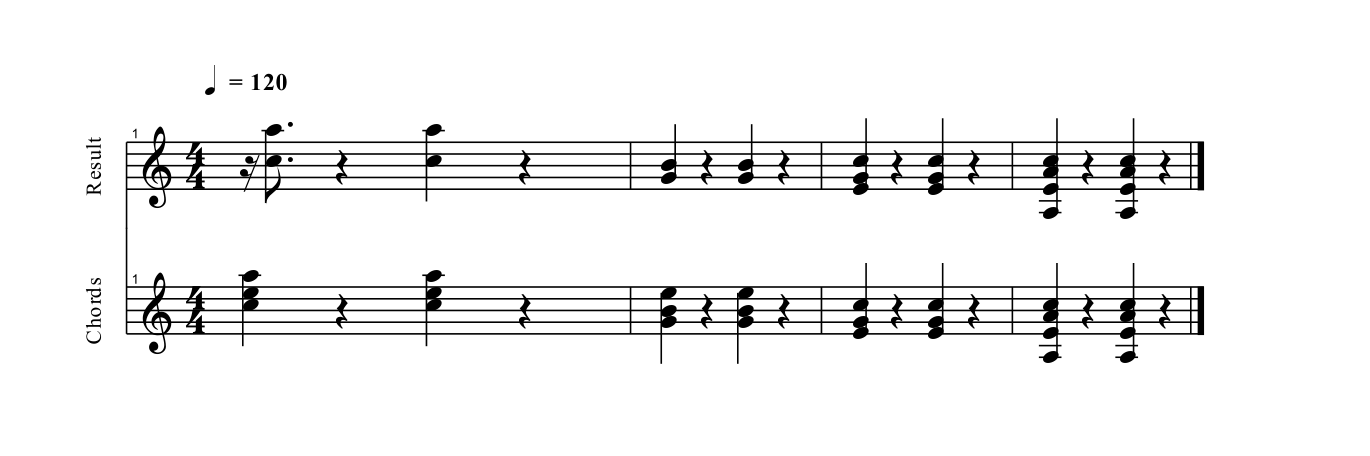
\includegraphics[width = 0.95\textwidth]{Am_chords_-_compare-001.png}

            \end{center}

        \end{figure}
	\end{frame}

    \begin{frame}
	\frametitle{Результаты}
	   \begin{figure}[h!]
            \begin{center}
                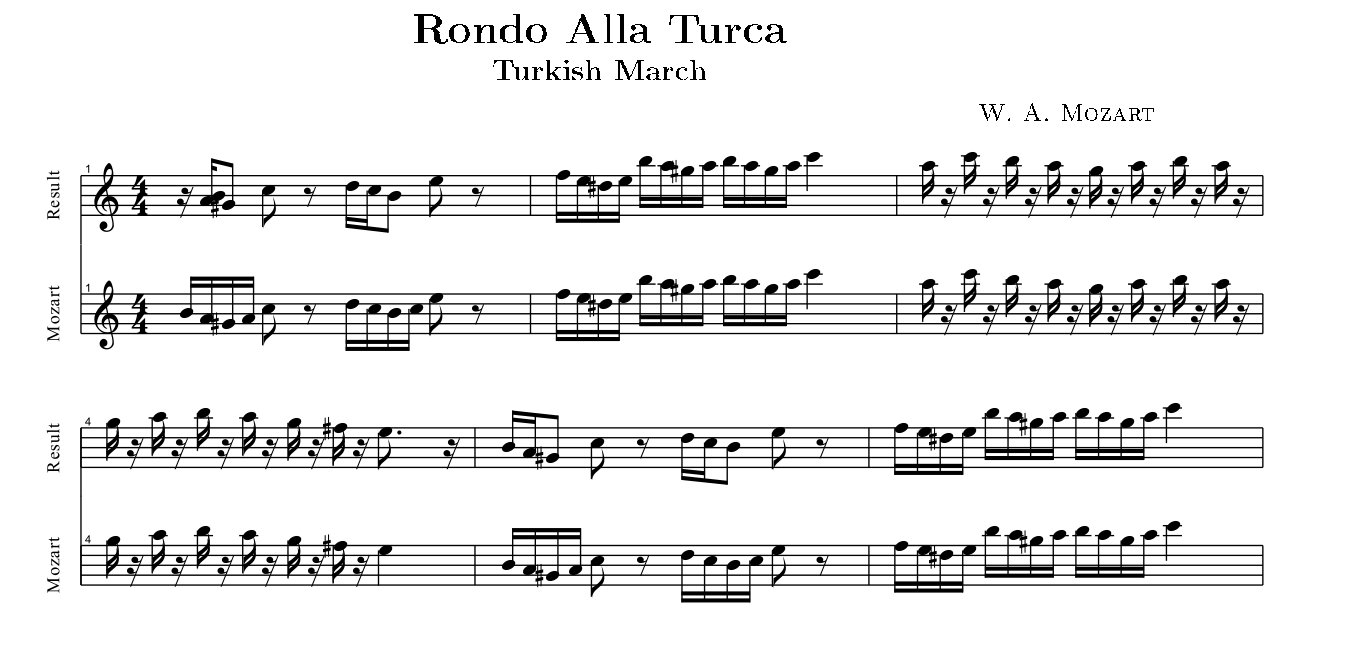
\includegraphics[width = 0.85\textwidth]{turca.png}
            \end{center}

        \end{figure}
	\end{frame}

    \begin{frame}
	\frametitle{Итоги}
%		Что использовалось:
	   \begin{figure}[t!]
            \begin{center}
                
\includegraphics[width =\textwidth]{logos.png}
            \end{center}
            \end{figure}
            
		Чему научились:
		\begin{itemize}
			\item Работа со звуковыми файлами
			\item Применение методов анализа временных рядов
		\end{itemize}
		Что дальше:
		\begin{itemize}
			\item Улучшение алгоритма
			\item Работа с микрофоном 
			\item Мобильное приложение
		\end{itemize}
	\end{frame}


    \begin{frame}
    \frametitle{Ссылки}
        \begin{itemize}
            \item \href{https://github.com/cscenter/uNotes.git}{https://github.com/cscenter/uNotes.git} - исходный код
            \item \href{polyakovdmi93@gmail.com}{polyakovdmi93@gmail.com} --- Денис~Поляков
            \item \href{vasdommes@gmail.com}{vasdommes@gmail.com}  --- Василий~Доммес
            \item \href{c.b.k@bk.ru}{c.b.k@bk.ru}  --- Сергей~Кривошеин
        \end{itemize}
	\end{frame}

\end{document} 